\begin{surferPage}{바스의 $6$차식}
    이 $6$차 곡면은 $1996$년에 울프 바스에 의해 만들어졌습니다. 
    
    이 곡면은 $65$개의 특이점을 갖습니다. 
%    (wenn man die $15$ im Bild nicht sichtbaren, ``unendlich fernen'', mitz�hlt)%
이는 바스가 식을 만든 직후 Jaffe와 Ruberman에 의해 $6$차식이 가질 수 있는 최대 개수라는 것이 증명되었습니다. 그러므로 이젠 누구도 바스의 기록을 깰 수 없죠!


바스의 발견은 사람들에게 큰 충격을 가져다주었습니다. 왜냐하면 꽤 오랜시간동안 $6$차식은 최대 $64$개의 특이점을 가진다고 믿어져 왔었기 때문입니다. 

이 곡면의 충격적인 특징은 정이십면체와 같은 대칭성을 갖는다는 것입니다. 아래의 그림은 정이십면체와 그것의 대칭면을 보여줍니다. 
%    Die Abb.\ zeigt diesen platonischen K�rper und seine Symmetrie - Ebenen: 
%    und diese Ebenen gemeinsam mit der Barth Sextik in einem Bild.     
    % 
  \begin{center}
      \vspace*{-0.1cm}
      \begin{tabular}{@{}c@{\ \ }c@{\,}c@{}}
        \begin{tabular}{@{}c}
          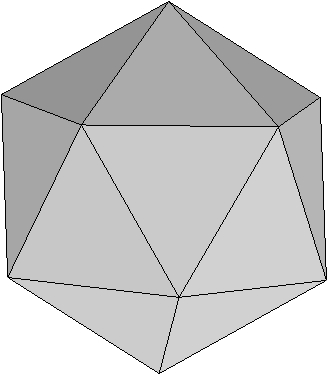
\includegraphics[width=1.4cm]{./../../common/images/icosah}
        \end{tabular}
        &
        \begin{tabular}{@{}c}
          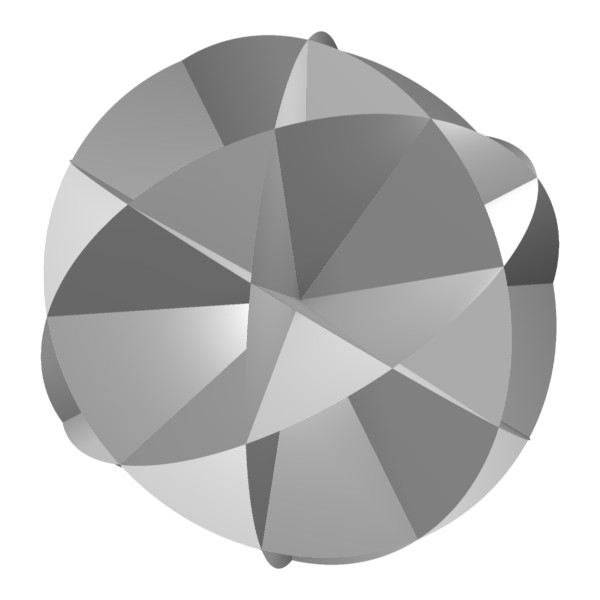
\includegraphics[width=1.4cm]{./../../common/images/barth_sextic_planes}
        \end{tabular}
        &
        \begin{tabular}{c@{}}
          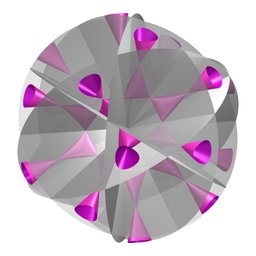
\includegraphics[width=1.4cm]{./../../common/images/barth_sextic_and_planes}
        \end{tabular}
      \end{tabular}
    \end{center}
    \vspace*{-0.1cm}

Barth의 $6$차식은 $P_6 - \alpha K^2=0$ 을 만족합니다. 여기서 $P_6$는 여섯개의 대칭면을 나타내고 $K=x^2+y^2+z^2-1$ 는 단위구를 나타냅니다. 마지막으로 $\alpha=\frac{1}{4}(2+\sqrt{5})$ 입니다.
\end{surferPage}
